\input ../SlidePreamble
\input ../preamble

\begin{document}

{\Huge

  \centerline{\bf TTIC 31230, Fundamentals of Deep Learning}
  \bigskip
  \centerline{David McAllester, Winter 2019}
  \vfill
  \centerline{\bf Language Modeling}
  \vfill
  \centerline{\bf Machine Translation}
  \vfill
  \centerline{\bf Attention}
  \vfill
  \centerline{\bf Beam Search}
  \vfill
  \centerline{\bf Statistical Machine Translation}

\slide{RNN for a generic CELL Procedure}
As usual, we use capital letter indeces to denote whole tensors or slices and lower case letters to denote particular index values.
\vfill
Procedure $\mathrm{RNN}_\Phi(x(T,I))$

\begin{eqnarray*}
h[0,J] &  = &  \mathrm{CELL}_{\Phi.\mathrm{cell}}(\Phi.\mathrm{init}[J],\;x[0,I]) \\
\mathrm{for}\;t>0\;\;h[t,J] &  =  & \mathrm{CELL}_{\Phi.\mathrm{cell}}(h[t-1,J],\;x[t,I])
\end{eqnarray*}

\vfill
Return $h[T,J]$



\slide{bi-directional RNNS}

\centerline{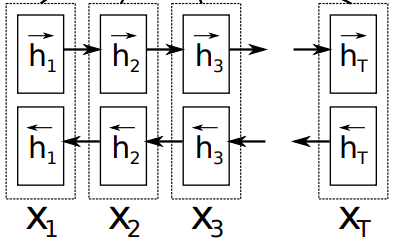
\includegraphics[width = 3in]{../images/biRNN}}

\begin{eqnarray*}
\vec{h}[T,J] & = & \vec{\mathrm{RNN}}_{\Phi.LR}(x[T,I]) \\
\\
\cev{h}[T,J] & = & \cev{\mathrm{RNN}}_{\Phi.RL}(x[T,I]) \\
\\
\mbox{for}\;t\;\;h[t,2J] & = & \vec{h}[t,J];\cev{h}[t,J]\;\;\mbox{where $x;y$ is vector concatenation}
\end{eqnarray*}


\slide{Multi-Layer RNNs}

\centerline{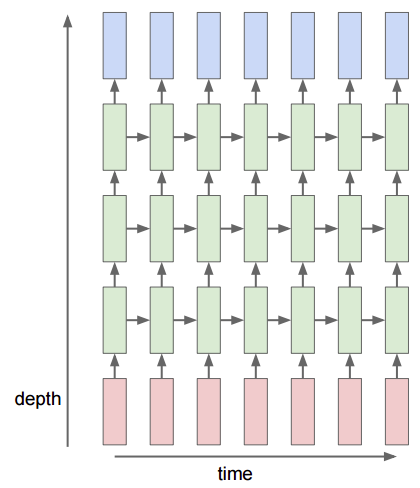
\includegraphics[width = 2in]{../images/RNNstack}}
\centerline{\large [Figure by Leonardo Araujo dos Santos]}

\begin{eqnarray*}
h[0,T,J] & = & \mathrm{RNN}_{\Phi[0]}(x[T,I]) \\
\\
\mbox{for} \;\ell > 0\;\;h[\ell,T,J] & = & \mathrm{RNN}_{\Phi[\ell]}(h[\ell-1,T,J])
\end{eqnarray*}

Each layer can be bidirectional.

\anaslide{Residual Multi-Layer RNNs}


\begin{eqnarray*}
h[0,T,J] & = & \mathrm{RNN}_{\Phi[0]}(x[T,I]) \\
\\
\mbox{for} \;\ell > 0\;\;h[\ell,T,J] & = & {\color{red} h[\ell-1,T,J] +} \mathrm{RNN}_{\Phi[\ell]}(h[\ell-1,T,J])
\end{eqnarray*}

\vfill
This is used in Google translation.

\slide{ Language Modeling}

Let $W$ be some finite vocabulary of tokens (words).

\vfill
Let $\mathrm{Pop}$ be a population distribution over $W^*$ (sentences).

\vfill
We will write a sequence $w[1],\ldots,w[t]$ as $w[T]$.

\vfill
We want to train a model $P_\Phi(w[T])$.

\begin{eqnarray*}
\Phi^* & = & \argmin_\Phi \; E_{\mathrm{Pop}}\;-\ln P_\Phi(w[T])
\end{eqnarray*}

\slide{The End of Sentence Token}

\vfill
We assume a special toeken {\tt <EOS>} called the end of sentence token.

\vfill
Let $t_{\mathrm{final}}$ be the last time index allowed for $T$.

\vfill
We requite $w[t_{\mathrm{final}}] = \mbox{\tt <EOS>}$ and $w[t] \not = \mbox{\tt <EOS>}$ for $t < t_{\mathrm{final}}$.

\vfill
This gives:

$$P(w[T]) = \prod_t\;P(w[t]\;|\;w[1],\ldots,w[t-1])$$

\slide{Autoregressive Models are Friendly}

I will call a model $P_\Phi(y)$ ``friendly'' if we can efficiently sample from $P_\Phi$ and we can also efficiently compute $P_\Phi(y)$ for any given $y$.

\vfill
Multiclass classification models for small $K$ are friendly.

\vfill
Gaussian distributions are friendly.

\vfill
Autoregressive language models are friendly --- they are a special case of friendly graphical models.

\vfill
General graphical models are often unfriendly.


\slide{Word Embeddings}

We will use a word embedding tensor $e[W,I]$ which should be interpreted as assigning a vector $e[w,I]$ to each word $w$.

\vfill
The word embedding tensor $e[W,I]$ is a parameter of language models (and many other kinds of NLP models).

\slide{Autoregressive Language Modeling}

Procedure $P_\Phi(w[T])$ ;; {\color{red} $w[T]$ given}

\vfill
{\huge \begin{eqnarray*}
x[t,I] & = & (\Phi.\mathrm{embed})[w[t],I] \\
\\
h[T,J] & = & \mathrm{RNN}_{\Phi.\mathrm{RNN}}(x[T,J])\;\;J \geq I \\
\\
s[0,w] & = & (\Phi.\mathrm{embed}[w,I]) \cdot (\Phi.\mathrm{init}[I]) \\
\\
\mathrm{for}\;t > 0\;\;s[t,w] & = & (\Phi.\mathrm{embed}[w,I]) \cdot h[t-1,I] \;\;\mbox{$h$ truncated to $I$} \\
\\
p[t,w] & = & \softmax_w\;s[t,w]
\end{eqnarray*}
}

\vfill
Return $\prod_t p[t,w[t]]$

\slide{Language Model Loss Decomposition}

\begin{eqnarray*}
\Phi^* &  = & \argmin_\Phi\; E_{\mathrm{Pop}} \;-\ln\;P_\Phi(w[T]) \\
\\
\\
\\
& = & \argmin_\Phi\;E_{\mathrm{Pop}}\;\sum_t\; -\ln\;p[t,w[t]]
\end{eqnarray*}

\slide{Standard Measures of Performance}

{\bf Bits per Character:}
For character language models performance is measured in bits per character.  Typical numbers are slightly over one bit per character.

\vfill
{\bf Perplexity:}
It would be natural to measure word language models in bits per word.  However, it is traditional to measure them in perplexity which is defined to be
$2^b$ where $b$ is bits per word.  Perplexities of about 60 are typical.

\vfill
According to Quora there are 4.79 letters per word.  1 bit per character (including space characters) gives a perplexity of $2^{5.79}$ or $55.3$.

\slide{Sampling From an Autoregressive Model}

To sample a sentence
\vfill
$$w_1,\ldots, w_T, \mbox{\tt <eos>}$$
\vfill
we sample $w_t$ from
\vfill
$$P_\Phi(w_t|w_1,\ldots,w_{t-1})$$

\vfill
until we get {\tt <eos>}.

\slide{Machine Translation}

%\centerline{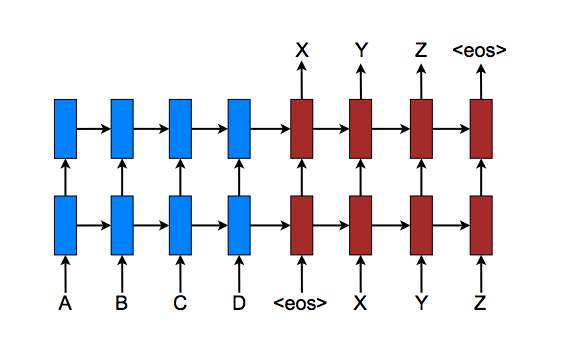
\includegraphics[width = 4in]{../images/SeqToSeq}}

%\centerline{\large [Figure from Luong et al.]}

$$w^{\mathrm{in}}_1,\ldots,w^{\mathrm{in}}_{t_{\mathrm{in}}} \Rightarrow w^{\mathrm{out}}_1,\ldots,w^{\mathrm{out}}_{t_{\mathrm{out}}}$$

$$w_{\mathrm{in}}[T_{\mathrm{in}}] \Rightarrow w_{\mathrm{out}}[T_{\mathrm{out}}]$$
\vfill
Translation is a {\bf sequence to sequence} (seq2seq) task.

\vfill
{\bf Sequence to Sequence Learning with Neural Networks}, Sutskever, Vinyals and Le, NIPS 2014, arXiv Sept 10, 2014.

\slide{Machine Translation}

%\centerline{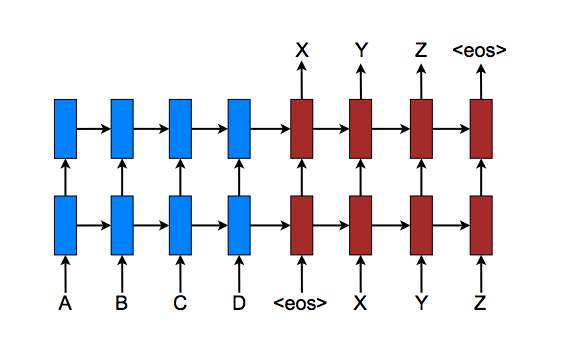
\includegraphics[width = 4in]{../images/SeqToSeq}}

%\centerline{\large [Figure from Luong et al.]}

$$w_{\mathrm{in}}[T_{\mathrm{in}}] \Rightarrow w_{\mathrm{out}}[T_{\mathrm{out}}]$$

\vfill
We define a model

\vfill
$$P_\Phi\left(w_{\mathrm{out}}[T_{\mathrm{out}}]\;|\; w_{\mathrm{in}}[T_\mathrm{in}]\right)$$

\vfill
\begin{eqnarray*}
\Phi^*  & = & \argmin_\Phi\; E_{\mathrm{Pop}} \;-\ln\;P_\Phi(w_{\mathrm{out}}[T_{\mathrm{out}}] \;|\; w_{\mathrm{in}}[T_{\mathrm{in}}]) \\
\\
& = & \argmin_\Phi \; E_{\mathrm{Pop}} \; -\ln P_\Phi(y|x)
\end{eqnarray*}


\slide{A Simple RNN Translation Model}

\vfill
We construct a conditional language model

\begin{eqnarray*}
\mathrm{Init}[J] & = & {\color{red} \cev{\mathrm{RNN}}_{\Phi.\mathrm{in}}(w_{\mathrm{in}}[T_{\mathrm{in}}])\;[0,J]} \\
\\
P_\Phi(w_{\mathrm{out}}[T_{\mathrm{out}}]\; | \; w_{\mathrm{in}}[T_{\mathrm{in}}]) & = & P_{\Phi.\mathrm{out}}(w_{\mathrm{out}}[T_{\mathrm{out}}] \;|\;\mathrm{Init}[J])
\end{eqnarray*}

\vfill
Here {\color{red} $\cev{\mathrm{RNN}}_{\Phi.\mathrm{in}}(w_{\mathrm{in}}[T_{\mathrm{in}}])\;[0,J]$} is used as the initial hidden state of an RNN language model for the output.

\vfill
{\color{red} $\cev{\mathrm{RNN}}_{\Phi.\mathrm{in}}(w_{\mathrm{in}}[T_{\mathrm{in}}])\;[0,J]$} is a ``thought vector'' representation of the input sentence.

\slide{Reverse Order Encoding}

Having the encoding run in the reverse order of the decoding helps in training by making it easier to start the translation correctly
(assuming that the languages have similar word orders).

\vfill
In the original paper the encoding was done left to right and the decoding was done right to left.

\slide{Machine Translation Decoding}

We can sample from $P_{\Phi.\mathrm{out}}(w[T]\;|\;H[J])$.

\vfill
But we might prefer

\begin{eqnarray*}
w_{\mathrm{out}}[T_{\mathrm{out}}]
& = & \argmax_{w_{\mathrm{out}}[T_{\mathrm{out}}]} \;P_\Phi\left(w_{\mathrm{out}}[T_{\mathrm{out}}] \;|\; w_{\mathrm{in}}[T_{\mathrm{in}}] \right)
\end{eqnarray*}

\vfill
This is typically approximated with greedy decoding:

\vfill
$$w_{\mathrm{out}}[t+1] = \argmax_w\; p_{\mathrm{out}}[t+1,w]$$

\vfill
These are not the same.

\slide{Attention-Based Translation}

{\bf Neural Machine Translation by Jointly Learning to Align and Translate}
Dzmitry Bahdanau, Kyunghyun Cho, Yoshua Bengio, ICLR 2015 (arXiv Sept. 1, 2014)

\vfill
There are many ways to construct attention-based translation models.

\vfill
Details are often unimportant.

\vfill
The model presented in these slides has been optimized for simplicity.


\slide{Representing Sentences by Vector Sequences}

The input sentence is now represented by a sequence of vectors.

\vfill
\begin{eqnarray*}
 & & P_\Phi(w_{\mathrm{out}}[T_{\mathrm{out}}] \;|\; w_{\mathrm{in}}[T_{\mathrm{in}}]) \\
 \\
& = & P_{\Phi.\mathrm{out}}(w_{\mathrm{out}}[T_{\mathrm{out}}]\;|\;
{\color{red} \cev{\mathrm{RNN}}_{\Phi.\mathrm{RNN}}(w_{\mathrm{in}}[T_{\mathrm{in}}])})
\end{eqnarray*}

\vfill
We still use {\color{red} $\cev{\mathrm{RNN}}_{\Phi.\mathrm{RNN}}(w_{\mathrm{in}}[T_{\mathrm{in}}])\;[0,J]$} as the initial state of a decoding RNN.

\vfill
But the decoding RNN now has access to the entire sequence of hidden states for the input.

\slidetwo{Attention-Based Translation}{Memory-Based Language Modeling}

Procedure $P_\Phi(w[T] \;|\; {\color{red} M[T_M,J]})$ ;;{\color{red} $w[T]$ given}
{\huge \begin{eqnarray*}
x[t,I] & = & (\Phi.\mathrm{embed})[w[t],I] \\
h[T,J] & = & \mathrm{RNN}_{\Phi.\mathrm{RNN}}(x[T,I] \;|\;{\color{red} M[T_M,J]})\;\;J \geq I \\
s[0,w] & = & (\Phi.\mathrm{embed}[w,I])\cdot (\Phi.\mathrm{init}[I]) \\
\mathrm{for}\;t > 0\;\;s[t,w] & = & (\Phi.\mathrm{embed}[w,I]) \cdot h[t-1,I] \;\;\mbox{$h$ truncated to $I$}\\
p[t,w] & = & \softmax_w\;s[t,w]
\end{eqnarray*}
}
Return $\prod_t p[t,w[t]]$

\slide{Attention-Based (Memory-Based) Conditional RNN}

Procedure $\mathrm{RNN}_\Phi(x[T_x,I] \;|\; {\color{red} M[T_M,J]})$

\begin{eqnarray*}
h[0,J] & = & \mathrm{CELL}_\Phi({\color{red} M[0,J]};x[t,I];{\color{red} 0[J]}) \\
\\
\mbox{for}\;t > 0\;\\
h[t,J] & = & \mathrm{CELL}_\Phi(\;{\color{red} h[t-1,J]};x[t,I];{\color{red}\mathrm{Lookup}(h[t-1,J],M[T,J])}\;)\\
\end{eqnarray*}

Return $h[T,I]$

\slide{Attention as a Key-Value Memory Mechanism}

Procedure $\mathrm{Lookup}(\mathrm{key}[J],\;M[T,J])$

\bigskip
\begin{eqnarray*}
s[t] & = &\mathrm{key}[J]^\top M[t,J] \\
\\
{\color{red} \alpha[t]} & {\color{red} =} & {\color{red} \softmax_t \;s[t]\;\mbox{; the attention}} \\
\\
{\color{red} V[J]} & {\color{red} =} & {\color{red} \sum_t\;\alpha[t]M[t,J]}
\end{eqnarray*}

\bigskip
Return $V[J]$



\slideplain{Attention in Image Captioning}

\centerline{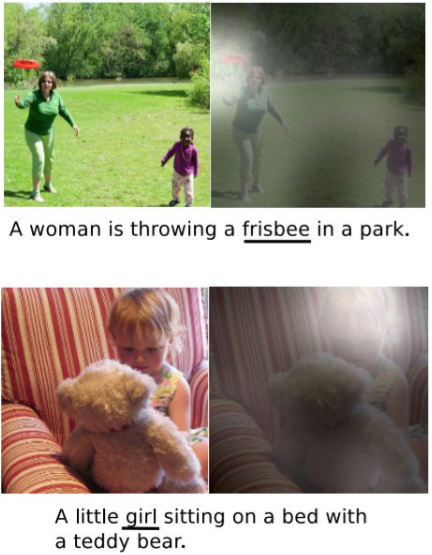
\includegraphics[width = 4in]{../images/AttentionInCaptioning1}}
\centerline{Xu et al. ICML 2015}

\slideplain{Greedy Decoding vs. Beam Search}

We would like

\vfill
$$W_{\mathrm{out}}[T_{\mathrm{out}}]^* = \argmax_{W_{\mathrm{out}}[T_{\mathrm{out}}]}
P_\Phi(W_{\mathrm{out}}[T_{\mathrm{out}}] \;|\;W_{\mathrm{in}}[T_{\mathrm{in}}])$$

\vfill
But a greedy algorithm may do well

\vfill
$$w_t = \argmax_w\; P_\Phi(w\;|\;W_{\mathrm{in}}[T_{\mathrm{in}}],\;w_1,\ldots,w_{t-1})$$

\vfill
But these are not the same.

\slide{Example}

``Those apples are good'' vs. ``Apples are good''

\vfill
$$P_\Phi(\mbox{Apples are Good {\tt <eos>}}) > P_\Phi(\mbox{Those apples are good {\tt <eos>}})$$

\vfill
$$P_\Phi(\mbox{Those}|\varepsilon) > P_\Phi(\mbox{Apples}|\varepsilon)$$
    
\slide{Beam Search}

At each time step we maintain a list the $K$ best words and their associated hidden vectors.

\vfill
This can be used to produce a list of $k$ ``best'' decodings which can then be compared to select
the most likely one.

\slideplain{Phrase Based Statistical Machine Translation (SMT)}

Step I:   Learn a phrase table --- a set of triples $(p,q,s)$ where

\vfill
\begin{itemize}
\item $p$ is a (short) sequence of source words.
  \vfill
\item $q$ is a (short) sequence of target words.
  \vfill
\item $s$ is a score.
\end{itemize}

\vfill
(``au'', ``to the'', .5) \hfill (``au banque'', ``for the bank'', .01)

\vfill
For a phrase triple $P$ we will write $P.\mathrm{source}$ for the source phrase, $P.\mathrm{target}$ for the target phrase, and $P.\mathrm{score}$ for the score.

\slide{Derivations}

Consider an input sentence $x$ of length $T$.

\vfill
We will write $x[s:t]$ for the substring $x[s]$, $\ldots$, $x[t-1]$.

\vfill
A derivation $d$ from $x$ is a sequence $(P_1,s_1,t_1,)$, $\ldots$, $(P_K,s_K,t_K)$ where $P_k.\mathrm{source} = x[s_k:t_k]$.

\vfill
The substrings $x[s_k:t_k]$ should be disjoint and ``cover'' $x$.

\vfill
For $d = [(P_1,s_1,t_1,)$, $\ldots$, $(P_L,s_K,t_K)]$ we define

$$ y(d) \equiv P_1.\mathrm{target}\;\cdots P_K.\mathrm{target}$$

\vfill
We let $D(x)$ be the set of derivations from $x$.

\slide{Scoring}

For $d \in D(x)$ we define a score $s(d)$

\vfill
$$s(d) = \alpha \ln P_\mathrm{LM}(y(d)) + \beta \sum_k P_k.\mathrm{score} + \gamma \;\mathrm{distortion}(d)$$

\vfill
where $P_{\mathrm{LM}}(y)$ is the probability assigned to string $y$ under a language model for the target language

\vfill
and $\mathrm{distortion}(d)$ is a measure of consistency of word ordering between source and target strings as defined by
the indeces $(s_1,t_1)$, $\ldots$, $(s_K,t_K)$.

\slide{Translation}

\begin{eqnarray*}
  y(x) & = & y(d^*(x)) \\
  \\
  \\
  \\
  d^*(x) & = & \argmax_{d \in D(x)} \;s(d)
\end{eqnarray*}

\slide{END}
}
\end{document}
